\chapter{Combining Models}
\section{Introduction}
\begin{description}
	\item[\textbf{committees}] Train $L$ different models and then make predictions using the average of the predictions made by each model.
	\item[\textbf{boosting}] Train multiple models in sequence in which the error function used to train a particular model depends on the performance of the previous models.
	\item[\textbf{decision trees}] Different models are responsible for making predictions in different regions of input space.
	\item[\textbf{mixtures of experts}] Models are viewed as mixture distributions in which the component densities,as well as the mixing coefficients,are conditioned on the input variables.
	\begin{align}
	p(t|\vec{x})=\sum\limits_{k=1}^{K}\pi_k(\vec{x})p(t|\vec{x},k)
	\end{align}
	in which $\pi_k(\vec{x})=p(k|\vec{x})$ represents the input-dependent mixing coefficients,and $k$ indexes the model.
\end{description}

\section{Bayesian Model Averaging}
In Bayesian model averaging the whole data set is generated by a single model.By contrast,when we combine multiple models,we see that different data points within the data set can potentially be generated from different values of the latent variable $\vec{z}$ and hence by different components.

\section{Committees}
The simplest way to construct a committee is to average the predictions of a set of individual models,to cancel the contribution arising from variance and bias.

\textbf{Bootstrap} data to introduce variability between the different models within the committee.Suppose we generate $M$ bootstrap data sets
\begin{align}
y_{COM}(\vec{x})=\dfrac{1}{M}\sum\limits_{m=1}^{M}y_m(\vec{x})
\end{align}
where $m=1,...,M$.This procedure is known as \textbf{bootstrap aggregation} or \textbf{bagging}.

\section{Boosting}
Here we describe the most widely used form of boosting algorithm:\textbf{AdaBoost},short for 'adaptive boosting'.The base classifiers are known as \textbf{weak learners} and are trained in \textbf{sequence} using a \textbf{weighted form of the data set} in which the weighting coefficient associated with each data point depends on the performance of the previous classifiers.

Consider a two-class classification problem,in which the training data comprises input vectors $\vec{x}_1,...,\vec{x}_N$ along with corresponding binary target variables $t_1,...,t_N$ where $t_n\in \{-1,1\}$.Each data point is given an associated weighting parameter $w_n$,initially set $1/N$ for all.A base classifier function $y(\vec{x})\in \{-1,1\}$
\begin{SCfigure*}
	\caption{Shematic illustration of boosting framework}
	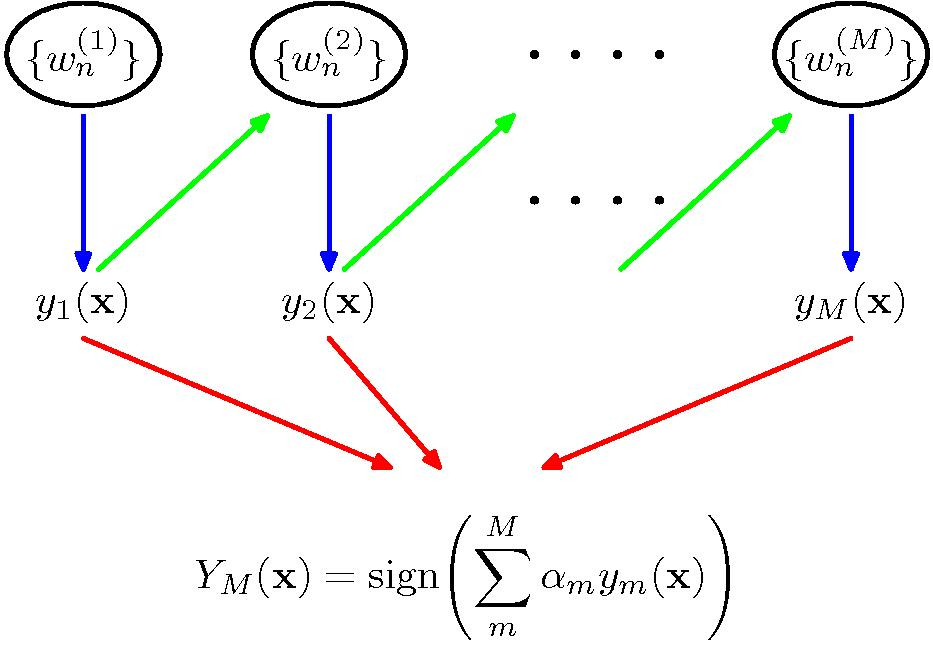
\includegraphics{prml/Figure14.1}
\end{SCfigure*}

\begin{algorithm}[H]
	\caption{\color{red}{AdaBoost}}
	\label{algo:AdaBoost}
	\DontPrintSemicolon % Some LaTeX compilers require you to use \dontprintsemicolon instead 
	\KwIn{A set $\vec{X} = \{\vec{x}_1, \vec{x}_2, \ldots, \vec{x}_N\}$,$\{t_1,...,t_N\}$}
	\KwOut{$y(\vec{x})$,.}
	1. Initialize the data weighting coefficients $\{w_n\}$ by setting $w_n^{1}=1/N$ for $n=1,...,N$. \;
	2. \For{$m=1,...,N$}{
		(a) Fit a classifier $y_m(\vec{x})$ to the training data by minimizing the weighted error function
		\begin{align}
		J_m=\sum\limits_{n=1}^{N}w_n^{(m)}I(y_m(\vec{x}_n)\neq t_n)
		\end{align}
		where $I(y_m(\vec{x}_n)\neq t_n)$ is the indicator function and equals $1$ when $y_m(\vec{x}_n)= t_n$ and $0$ otherwise. \;
		(b) Evaluate  the quantities
		\begin{align}
		\epsilon_m=\dfrac{\sum_{n=1}^{N}w_n^{(m)}I(y_m(\vec{x}_n)\neq t_n)}{\sum_{n=1}^{N}w_n^{(m)}}
		\end{align}
		and then use these to evaluate
		\begin{align}
		\alpha_m=\ln\{\dfrac{1-\epsilon_m}{\epsilon_m}\}.
		\end{align}
		\;
		(c) Update the data weighting coefficients
		\begin{align}
		w_n^{(m+1)}=w_n^{(m)}\exp\{\alpha_m I(y_m(\vec{x}_m)\neq t_n)\}
		\end{align}
	}
	3. Make predictions using the final model,which is given by
	\begin{align}
	Y_M(\vec{x})=sign(\sum_{m=1}^{M}\alpha_m y_m(\vec{x}))
	\end{align}
		
\end{algorithm}

\subsection{Minimizing exponential error}
Consider the exponential error function defined by
\begin{align}
E=\sum_{n=1}^{N}\exp\{-t_n f_m(\vec{x}_n)\}
\end{align}
where $f_m(\vec{x})$ is a classifier defined in terms of a linear combination of base classifiers $y_l(\vec{x})$ of the form
\begin{align}
f_m(\vec{x})=\dfrac{1}{2}\sum_{l=1}^{m}\alpha_l y_l(\vec{x})
\end{align}
and $t_n\in \{-1,1\}$ are the training set target values.Our goal is to minimize $E$ with respect to the weighting coefficients $\alpha_l$ and parameters of the base classifiers $y_l(\vec{x})$.

Separating off the contribution from base classifier $y_m(\vec{x})$,
\begin{align}
E&=\sum_{n=1}^{N}\exp\{-t_n f_m(\vec{x}_n)\} \\
&=\sum_{n=1}^{N}\exp\{-t_n \dfrac{1}{2}\sum_{l=1}^{m}\alpha_l y_l(\vec{x}) \} \\
&=\sum_{n=1}^{N}\exp\{-t_n f_{m-1}(\vec{x}_n)-\dfrac{1}{2}t_n \alpha_m y_m(\vec{x}_n)\} \\
&=\sum_{n=1}^{N}w_n^{(m)}\exp\{-\dfrac{1}{2}t_n \alpha_m y_m(\vec{x}_n)\}
\end{align}
where the coefficients $w_n^{(m)}=\exp\{-t_n f_{m-1}(\vec{x}_n)\}$ can be viewed as constants because we are optimizing only $\alpha_m$ and $y_m(\vec{x})$.Denote by $\mathcal{T}_m$ the set of data points correctly classified by $y_m(\vec{x})$ and misclassified points by $\mathcal{M}_m$,then we in turn rewrite the error function
\begin{align}
E &=e^{-\alpha_m/2}\sum_{n\in\mathcal{T}_m}w_n^{(m)}+e^{\alpha_m/2}\sum_{n\in\mathcal{M}_m}w_n^{(m)} \\
&=(e^{\alpha_m/2}-e^{-\alpha_m/2})\sum_{n=1}^{N}w_n^{(m)}I(y_m(\vec{x}_n)\neq t_n)+e^{-\alpha_m/2}\sum_{n=1}^{N}w_n^{(m)}
\end{align}
Then we can minimize this with respect to $y_m(\vec{x}_n)$ and $\alpha_m$.
\begin{align}
\because w_n^{(m)}=\exp\{-t_n f_{m-1}(\vec{x}_n)\} \\
\therefore w_n^{(m+1)}=\exp\{-t_n f_{m}(\vec{x}_n)\} \\
\therefore w_n^{(m+1)}=w_n^{(m)}\exp\{-\dfrac{1}{2}t_n\alpha_m y_m(\vec{x}_n)\}
\end{align}
Making use of the fact that
\begin{align}
t_n y_m(\vec{x})=1-2I(y_m(\vec{x}_n)\neq t_n)
\end{align}
we see updates at the next iteration
\begin{align}
w_n^{(m+1)}=w_n^{(m)}\exp(-\alpha_m/2)\exp\{\alpha_m I(y_m(\vec{x}_n)\neq t_n)\}
\end{align}
Because the term $\exp(-\alpha_m/2)$ is independent of $n$,so can be discarded.

\subsection{Error functions for boosting}



\section{Tree-based Models}






\section{Conditional Mixture Models}




























